\documentclass{llncs}

\usepackage{booktabs}
\usepackage[ruled]{algorithm2e} % For algorithms

\usepackage{siunitx}
\usepackage{graphicx}
\usepackage{multirow}
\usepackage[caption=false]{subfig}
\usepackage[capitalise]{cleveref}
\usepackage{todonotes}

\begin{document}

\title{Viability of Bone-Conduction and Spatialised Audio to Provide Guidance Instructions for People with Visual Impairments}
\titlerunning{Guiding People with Bone-Conduction and Spatialised Audio}

\author{Jacobus C. Lock\inst{1} \and 
Iain Gilchrist\inst{2} \and
Grzegorz Cielniak\inst{1} \and
Nicola Bellotto\inst{1}}

\institute{University of Lincoln \email{\{jlock, gcielniak, nbellotto\}@lincoln.ac.uk} \url{https://lcas.github.io/ActiVis/} \and
	   University of Bristol \email{i.d.gilchrist@bristol.ac.uk}}

\authorrunning{Jacobus C. Lock et.\ al.}

\maketitle
\setcounter{footnote}{0}

\begin{abstract}
  The ActiVis project is attempting to build a mobile guidance aid to help people with limited vision find objects in an unknown environment.
  This system uses bone-conducting headphones to transmit audio signals to the user and requires an effective non-visual interface.
  To this end, we propose an audio-based interface that uses a spatialised signal to convey a target's position on the horizontal plane. 
  The position on the median plan is given by adjusting the tone's pitch to overcome the audio localisation limitations of bone-conducting headphones. 
  This interface is validated through a set of experiments. 
\keywords{Human-machine interface \and vision impairment \and spatialised sound \and varying pitch \and bone-conduction}
\end{abstract} 

\section{Introduction}

In recent years, governments have spearheaded numerous initiatives to support people with disabilities and enable them to play a more active role in modern society.
The UK's Royal National Institute of Blind People (RNIB) for example has prioritised improving access to everyday services and products, such as public transport and mobile apps~\cite{rnib2016uk}.
Improvements in modern computing have made it possible for new and innovative solutions to these problems to come to the fore.
In particular, researchers in the active vision field have have made much progress in enabling machines to autonomously manipulate cameras to gather information about an environment for mapping, as well as object and object finding tasks~\cite{bajcsy2018revisiting}.
There is, however, a significant research question about whether techniques from active machine vision can be applied to humans, i.e.\ can a machine identify a point of interest in a scene and direct a human, instead of an electronic servo, to focus on that point?
If this can be done, it would be beneficial to people with visual impairments and will augment their ability to search for an arbitrary point or object of interest and identify an unknown scene. 

The ActiVis project aims to deliver a mobile guidance system based on the Google Project Tango platform~\footnote{\url{https://en.wikipedia.org/wiki/Tango\_(platform)}}, pictured in \cref{fig:tango-headphone}, that will ultimately be able to guide a user with vision impairments on the last leg of their journey, i.e.\ the so-called `last 10-yard problem'. 
The entire platform is based on a Google Project Tango device that provides access to powerful real-time localisation (through IMU measurements and landmark tracking) and image-processing facilities and provides access to Android's full range of interface tools and IO options. 
Furthermore, a set of bone-conducting headphones (pictured in \cref{fig:tango-headphone}), that are placed on a user's cheekbones instead of their ears and do not interfere with normal hearing, are used to transmit the audio signals to the user.

\begin{figure}[t]
  \centering
  \subfloat[]{\label{fig:tango-headphone}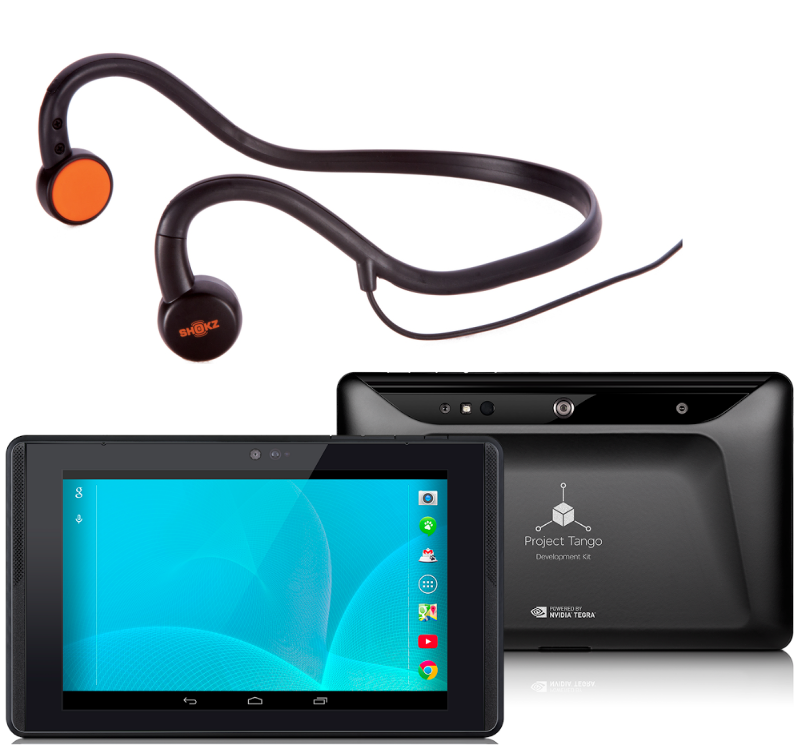
\includegraphics[width=0.4\columnwidth]{figures/tango_headphone.png}}
~
  \subfloat[]{\label{fig:participant}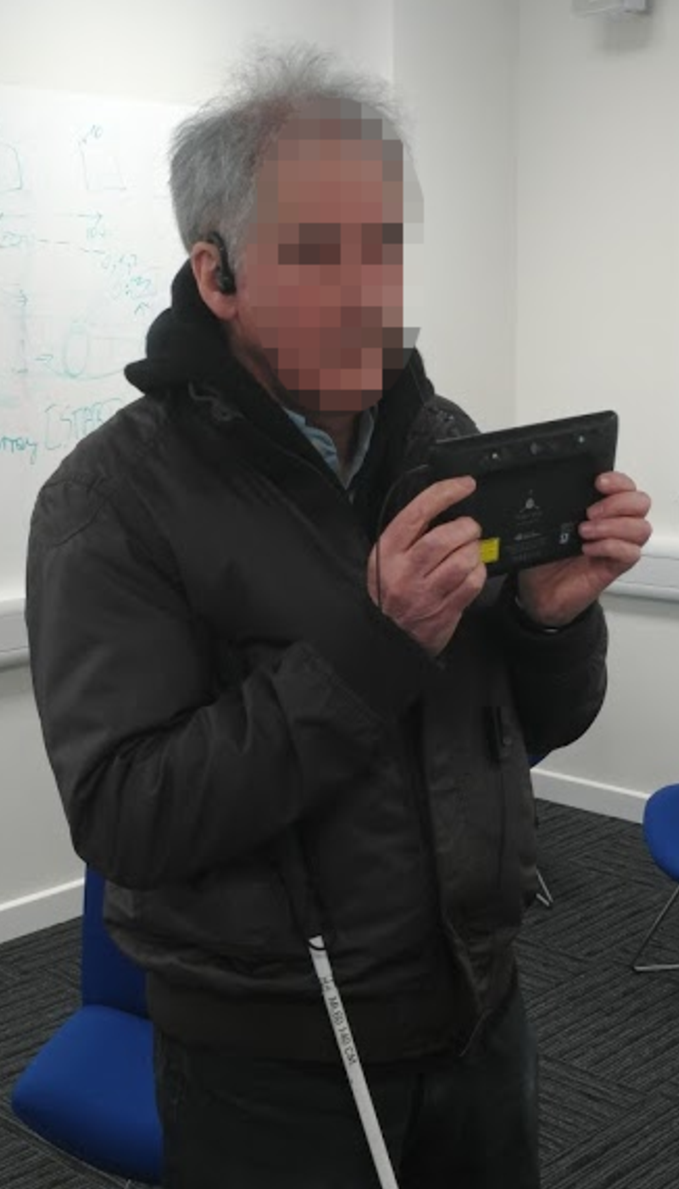
\includegraphics[width=0.25\columnwidth]{figures/vi_participant.pdf}}
  \caption{Pictures of the Tango device and bone-conducting headphones the system is based on (left) and both in use in an experiment (right).}
\end{figure}

Humans are able to determine the 3D position of a sound source and by exploiting this natural ability, the real-time guidance instructions can easily be interpreted without posing a significant cognitive load.
A sound source can be spatialised by adjusting a tone's spectral make-up (elevation angle), time delay and level difference (pan angle) and intensity (distance).
In this case, only the pan and elevation positions are transmitted.
However, since bone-conducting headphones bypass the outer ear structure, their spectral signature cannot properly be interpreted and we therefore convey the target's elevation angle by adjusting the tone's pitch.
A similar approach was used in~\cite{durette2008visuo}, but the study did not focus on or investigate the interface's efficacy.
Indeed, this work serves as an initial study into an interface that can effectively communicate the pan and elevation angles of a target location through a set of bone-conducting headphones using standard audio libraries and audio manipulations.
Furthermore, we demonstrate this approach's effectiveness through a simple experiment.

The rest of the paper starts off by discussing previous relevant works and research in \cref{sec:prev-work}, followed by a discussion on the design and implementation of our interface in \cref{sec:interface-design}.
This is followed by a description of the experiments that were conducted and a discussion of their results in \cref{sec:experiment-and-results}.
Finally, the work is concluded with a summary and a short discussion on future research prospects in \cref{sec:conclusion}.

\section{Previous Work}\label{sec:prev-work}

Multiple mobile navigation and travel aids have been devised throughout the years, some as part of a commercial undertaking and many as part of academic research.
The majority of these systems rely on one or a combination of vocal~\cite{mocanu2016when,chessa2016integrated,kanwal2015navigation}, audio~\cite{schwarze2015intuitive,rodriguez2012obstacle,katz2010navig} and haptic~\cite{rivera-rubio2015assistive,lee2015rgb,xiao2015assistive} feedback media to communicate guidance instructions to the user, each with their own sets of features and limitations.
In general, participants with vision impairments report that they prefer haptic and vocal feedback out of the 3 options.\todo{ref blind preferences}
However, haptic feedback systems typically have extra hardware requirements to transmit the guidance instructions.
Furthermore, haptic and vocal feedback can become a cognitive burden, particularly where high resolution guidance, which can exceed the bandwidth of these particular senses, is required.
Indeed, participants report that they would prefer control over the vocal feedback channel and trigger guidance instructions, instead of being given constant guidance instructions. 
Simple audio tones do not suffer from these bandwidth and hardware limitations as badly, but it does have the potential to fatigue the user's senses if the tone is too harsh, psychologically speaking.

Researchers have investigated using audio signals that are spatialised with an HRTF, which tricks the brain into thinking that a sound source is located at some arbitrary 3D position~\cite{geronazzo2016interactive,wilson2007swan,katz2010navig,blum2013spatialized}.
The authors generally report favourable results for this guidance approach when used with standard over-ear headphones or speakers. 
However, other authors have found that the choice of audio transmission medium can have a significant effect on performance.
Cheaper headphones and bone-conduction headphones generally report unfavourable results when compared to over-ear or more expensive alternatives~\cite{schonstein2008comparison,macdonald2006spatial,stanley2006lateralization}. 
This seems to be limited to the elevation dimension, however, and can be improved with HRTFs adjusted for the bone-conduction pathway~\cite{stanley2006lateralization}.
In~\cite{durette2008visuo}, they transmit a target's elevation angle by adjusting the signal's pitch and report favourable results. 
However, these studies focussed on their system's total effectiveness, rather than the effectiveness of their pitch adjustment mechanism and in this work we endeavour to investigate this more closely. 

\section{Interface Description}\label{sec:interface-design}

\subsection{Hardware Selection}

Electronic navigation aids and guidance systems for people with vision impairments have had trouble appealing to the visually impaired community at large because of problems that are common of academic research and prototypes: prohibitive costs, unfriendly user interfaces and significant hardware requirements, e.g.\ head-mounted cameras and GPS antennae~\cite{golledge2004stated,yusif2016older,arditi2013user}.
Indeed, the traditional walking cane remains the go-to tool for navigation and obstacle avoidance. 
With the ActiVis system, we aim to tackle the issue of cost, user-acceptance and usability by using only `standard' devices and hardware as far as possible and avoiding any special requirements.
Following this design target, we base the project on a mobile device and discreet headset with the expectation that the user will not stand out if seen walking in public with a phone in their hand and wearing a headset.
The ActiVis system is based on a concept proposed in~\cite{bellotto2013multimodal,lock2017portable}, which uses a Google Tango device that is able to localise itself in real-time and generate and has the benefit of a compact, familiar form-factor which will help overcome the hurdle of user-acceptance and usability.

A set of bone-conducting headphones is used as the audio transmission medium.
These headphones sit on a user's cheekbones and conduct the audio signals through the skull into the inner ear, instead of through the outer ear like typical over-ear headphones do. 
This has the benefit of not denying the user access to ambient sounds and noise, which could prove dangerous to a person with limited vision that relies on sound to detect oncoming vehicles and people, for example~\cite{lichtenstein2012headphone}.
Open-back headphones that allow ambient noise through were also considered, but the AfterShockz headphones pictured in \cref{fig:tango-headphone} were ultimately selected since they do not interfere at all with incoming sound (open-back headphones are better than closed back ones in this regard, but still muffle incoming sound) and are also more discreet than the larger over-ear headphone models. 

\subsection{Human Audio Localisation}

Humans localise a sound source in 3 dimensions by considering cues recorded in one ear (monaural cues) and comparing cues received at both ears (binaural cues)~\cite{blauert1997spatial,blauert1969sound}.
The binaural cues include ITD and ILD that help to determine a source's location on the horizontal plane.
Monaural cues are taken from the interaction of the sound with the human anatomy, e.g.\ head, shoulders, outer ear, before it enters the ear canal.
%The user's anatomy acts as a filter and the direction the sound wave hits the body activates different filter resonances, attenuating or accentuating different frequency bands.
When the modified audio signal enters the inner ear canal, the human brain is able to analyse the frequency response and accurately determine the position of the sound source on the median plane. 
The distance to the source is simply derived as the intensity, or volume, of the source, i.e.\ a louder sound would appear closer to the user than a softer one does. 

When an audio signal is transmitted via a set of speakers or headsets, it can be transformed with an HRTF to mimic the characteristics of a natural sound source before it is transmitted, tricking the brain into believing a sound is located at some arbitrary position.
An HRTF is a mathematical function that simulates the response signal of a human head and is derived by capturing key characteristics that affect the monaural and binaural responses, such as the user's hearing levels and head size, etc.
Since hearing responses are unique amongst different users, the best results would be observed if each user had their own customised HRTF.\
However, given the complicated process involved to capture the required user characteristics, making unique HRTFs is often an untenable solution and using average values (e.g.\ head measurements, height, etc.) have shown to produce acceptable results~\cite{gardner1995hrtf}.

\subsection{Interface Design}

The guidance target is presented to the user in terms of pan and elevation angles, indicating the angle adjustments that are required to point the device camera at the target location, as shown in \cref{fig:cam-coords}.
Spatialised audio signals are well-suited to the task, displaying similar levels of performance to vocal feedback, but with less cognitive load and higher resolution~\cite{klatzky2006cognitive}.
However, the audio guidance signals are delivered to the user with a set of bone-conducting headphones that bypass the user's outer-ear structure and since this structure plays an important role in localising a sound source's elevation\cite{blauert1969sound}, an alternative mode of conveying the elevation angle is required.\todo{check repeating from hardware selection section}
Therefore, we propose a simple linear adjustment to the signal's pitch as a function of the elevation angle. 
The pan angle can be conveyed by transforming the audio signal with an HRTF, and indeed it has been found that this dimension is unaffected by using bone-conducting headphones\cite{schonstein2008comparison,macdonald2006spatial,stanley2006lateralization}. 

\begin{figure}
  \centering
  \subfloat[]{\label{fig:cam-coords}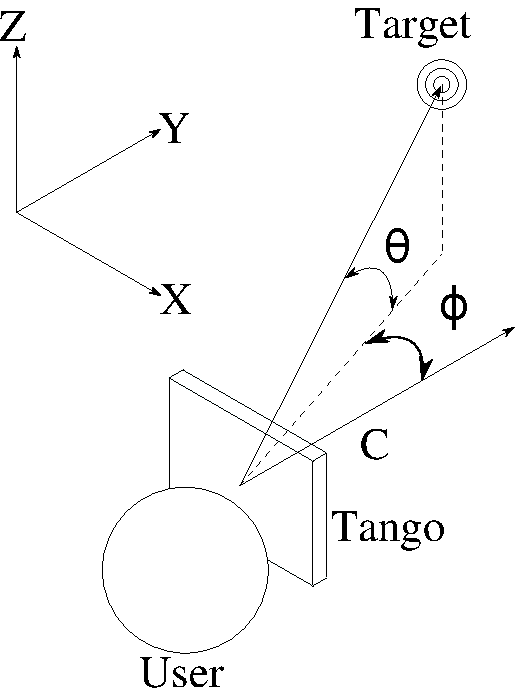
\includegraphics[width=0.3\columnwidth]{figures/camera_coordinate.pdf}}
~
  \subfloat[]{\label{fig:pitch-gain}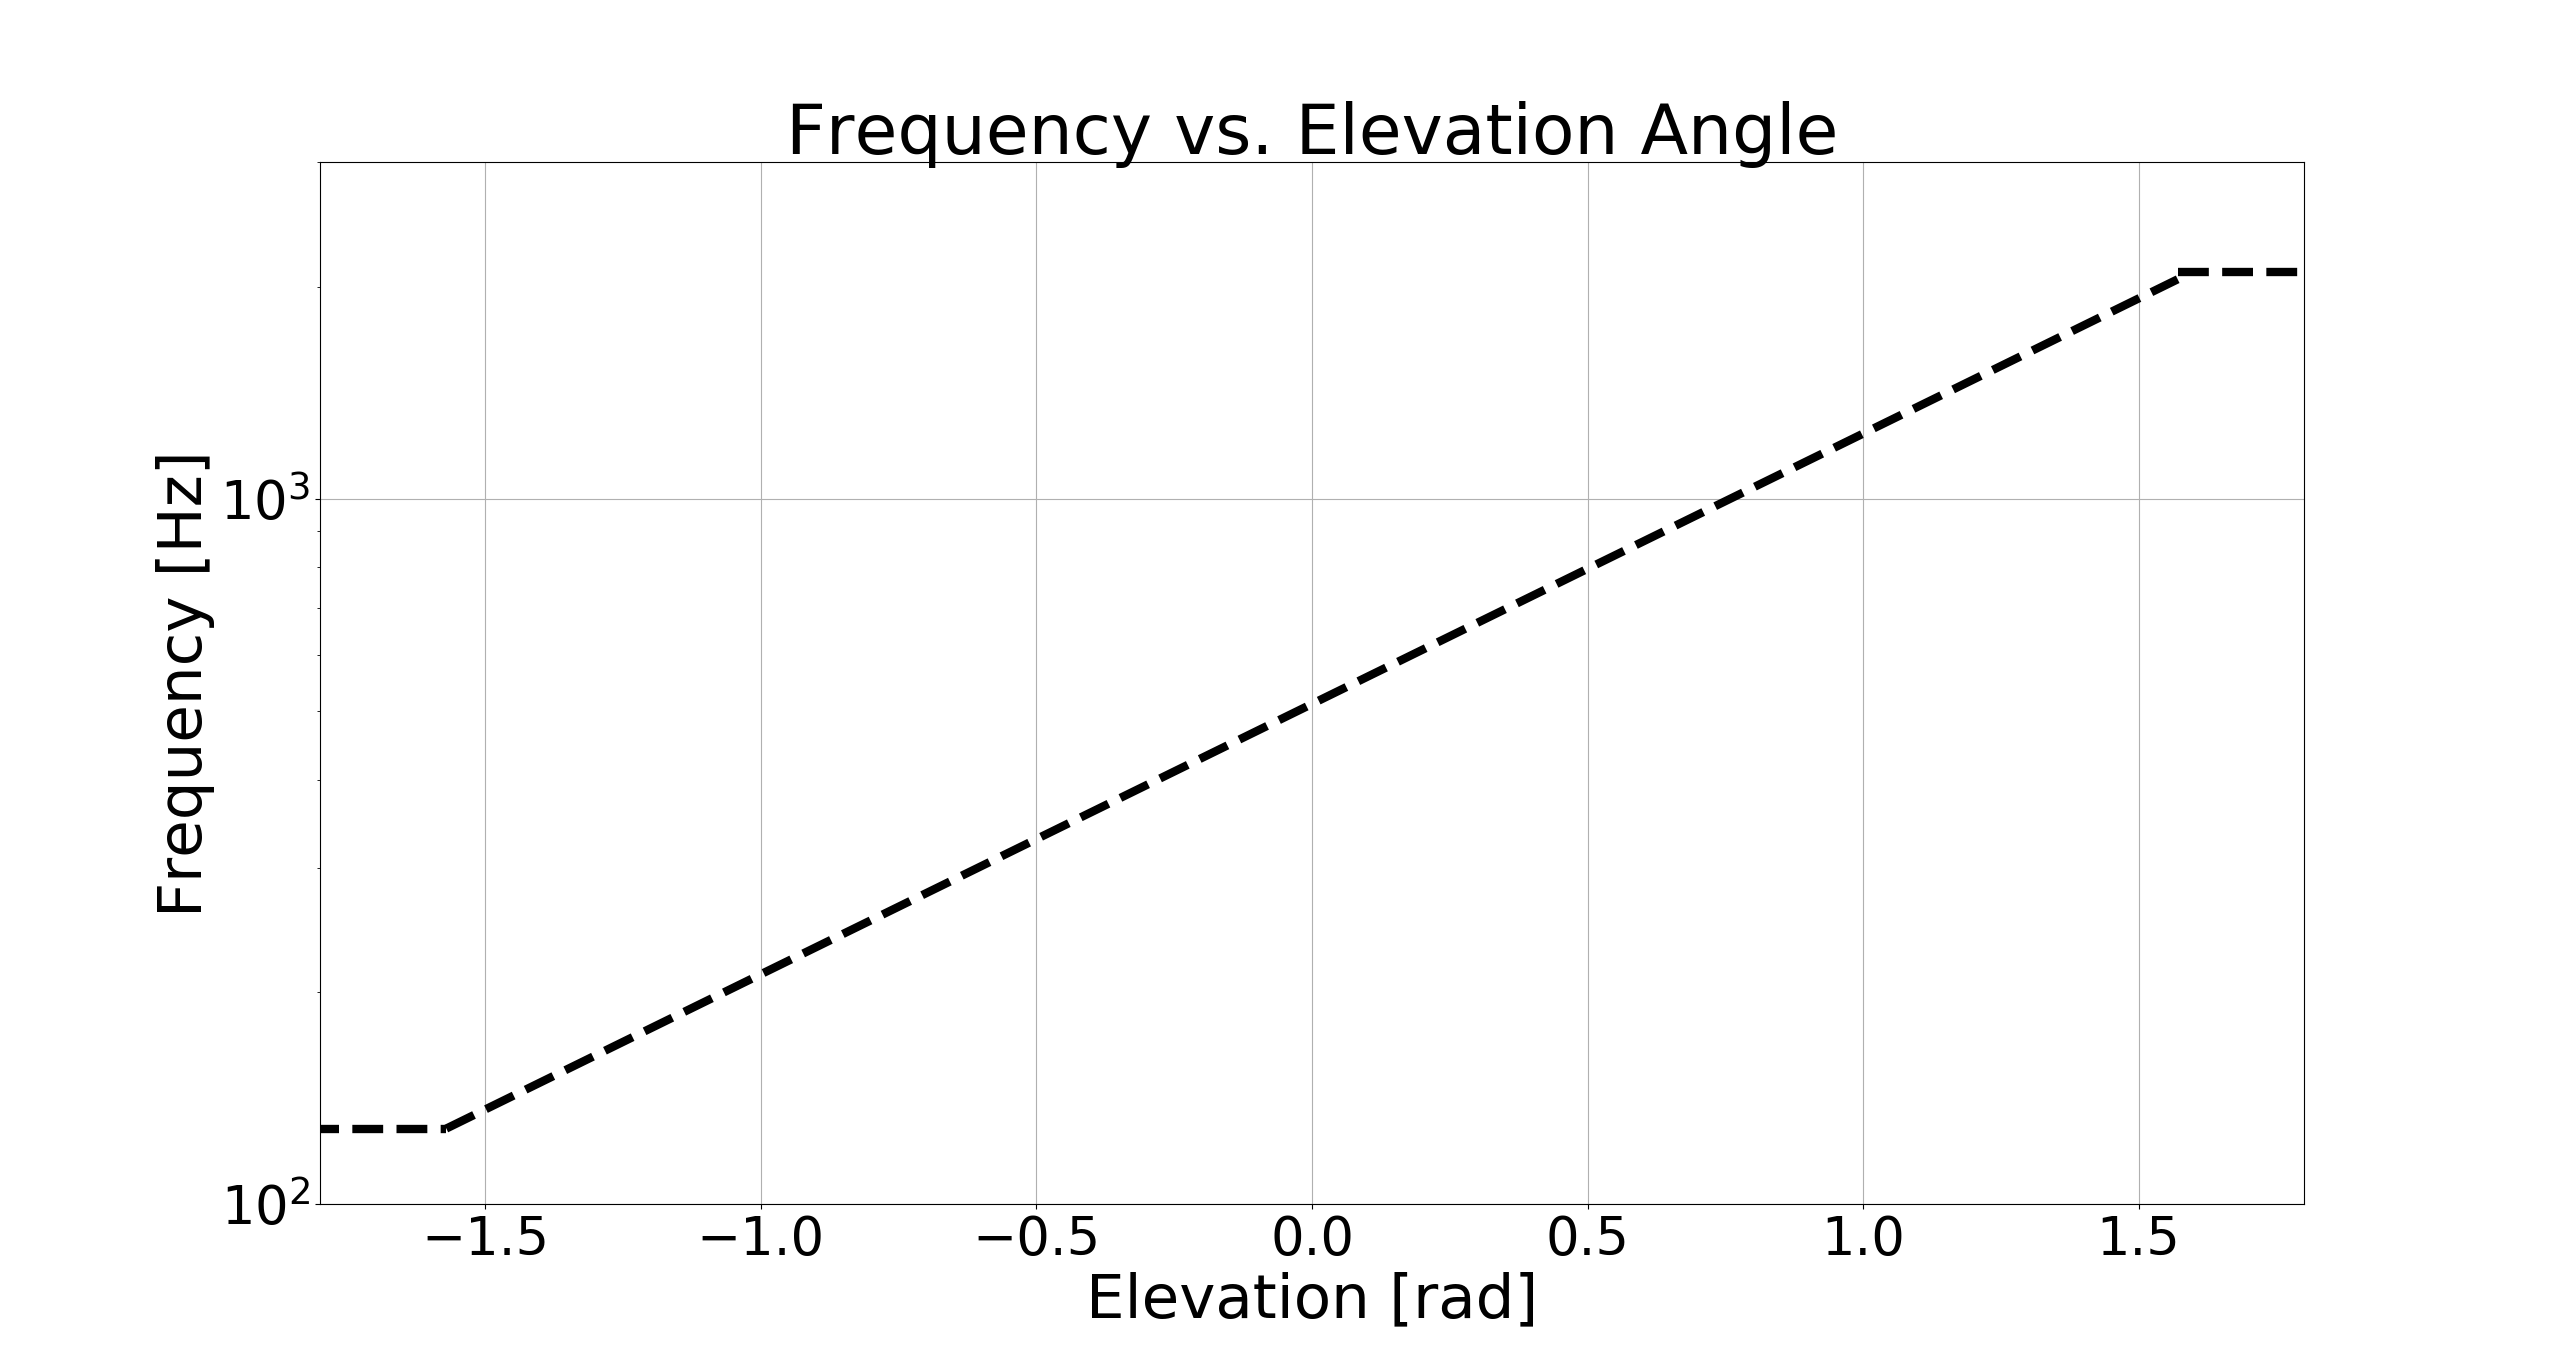
\includegraphics[clip, trim=0 0 0 40, width=0.6\columnwidth]{figures/pitch_gain_function.png}}
  \caption{The reference system used by the guidance interface showing the camera vector and pan and elevation angles (left) and the pitch gain function used to convey the target's elevation angle (right). }
\end{figure}

\subsubsection{Pan}

The human audition system uses binaural comparison cues, such as the inter-aural time and level differences (ITD and ILD respectively), to localise a sound source on the horizontal plane~\cite{blauert1969sound}.
The ITD is the perceived time delay between the signal reaching both ears, while the ILD is the perceived volume difference in the signal.
For example, a sound that comes from the individual's right, will hit the right ear first with a slightly higher volume.

In this work, a pure sinusoidal wave refreshed at \SI{10}{\hertz} was used. 
People typically have trouble localising a pure tone devoid of a rich spectral signature.
However, the ITD and ILD is independent of the tone's spectral make-up and the elevation angle is given through a different mechanism and a pure sine wave is therefore sufficient to convey the target's pan angle.
To transform and spatialise the audio signal, we used OpenAL's default HRTF, based on the MIT's KEMAR dataset~\cite{hiebert2005openal}, that uses the user and targets' positions as input and outputs a transformed audio signal.

\subsubsection{Elevation}

A generic HRTF implementation with bone-conducting headphones has trouble conveying the elevation angle of a sound source accurately~\cite{macdonald2006spatial,schonstein2008comparison}.
To compensate for this, we convey the target's elevation angle by adjusting the tone's pitch (i.e.\ the sine wave's frequency) as a function of the elevation. 
When the camera vector is at the target's elevation, the tone is set to neutral pitch.
Then, when the target is above the camera vector, the pitch is increased and decreased when the target is below the camera vector.
This high/low association scheme is used given humans' natural association of high-pitched sounds with elevated sound sources and lower-pitched sounds with source's below the individual's earline~\cite{pratt1930spatial,blauert1997spatial}.
A logarithmic, octave and semi-tone based function is used to adjust the tone's pitch to ensure perceptible changes while keeping the timbre roughly constant~\cite{shepard1964circularity}.
The pitch is updated at a rate of \SI{10}{\hertz} and changes as the user moves the device.

The pitch is changed as a linear function of the elevation angle and the gradient is determined by setting the angle and pitch limits.
For this work we only consider a \SI{180}{\degree} field of view in front of the user and limit the elevation angle to a range of $[-\frac{\pi}{2}, \frac{\pi}{2}]$.
The pitch limits are set at some integer number of octaves above and below the neutral, on-elevation pitch.
After practical tests with the interface, we set the neutral pitch to \SI{512}{\hertz}, which is comfortably audible and allows for a large number of audible octave limits to be selected.
For this work, we set the pitch limits to 2 octaves away from the neutral pitch, giving frequency limits of [\SI{128}{\hertz}, \SI{2048}{\hertz}].
The linear function is visualised in \cref{fig:pitch-gain}.

\subsection{Implementation}

A diagram of the experimental system pipeline is shown in \cref{fig:pipeline}, where the arrows indicate the direction of the flow of information.
When the user taps the Tango's screen, a new virtual target is generated and its coordinates are sent to the audio generation module, along with the device's current position and orientation.
The audio generator then produces a tone based on the difference between the device and target's positions and sends it to the audio output channel, which plays it back to the user.
The WiFi recording module is constantly monitoring the different parameter values of the device and target's positions, as well as the system's output, and records it to a remotely stored datafile. 

\begin{figure}
  \centering
  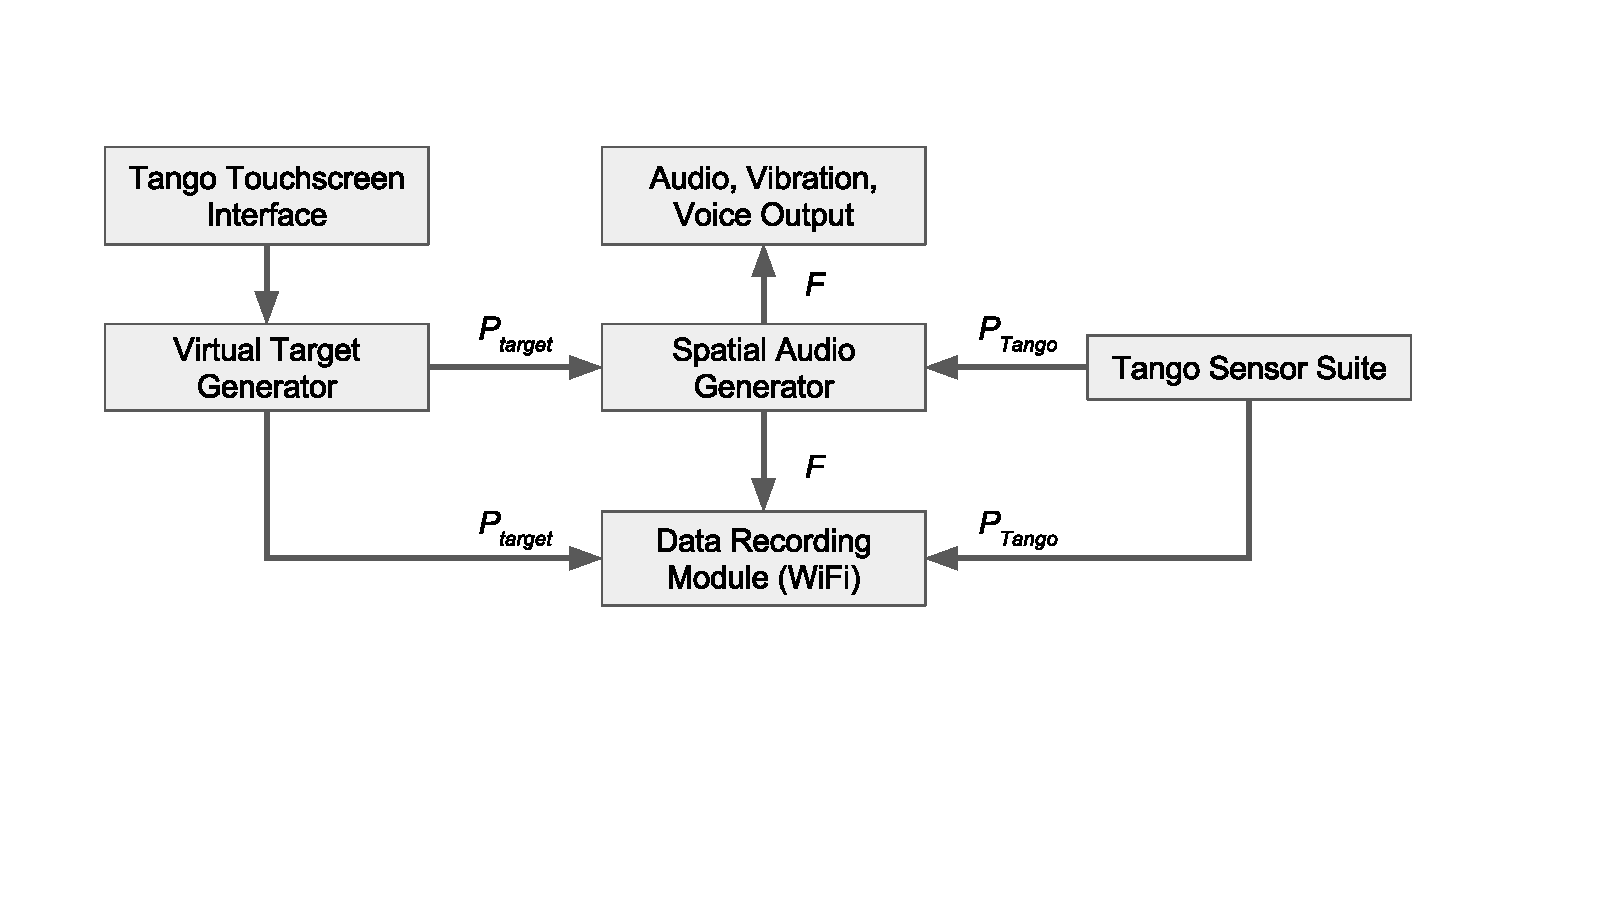
\includegraphics[clip=true, trim=0 120 80 50, width=0.8\columnwidth]{figures/pipeline.pdf}
  \caption{A diagram of the individual system components and their communication pipelines. $F$ indicates a feedback signal and $P$ a pose signal. }\label{fig:pipeline}
\end{figure}

\section{Experiment and Results}\label{sec:experiment-and-results}

\subsection{Procedure}

To test the interface's effectiveness at directing a user towards a target area, a set of experiments were conducted with a pointing task that is set up to capture the difference between the targets' actual position and the positions the participants' perceived them to be.
The participants are given a Tango tablet device running an app written for the experiment that generates a set of virtual targets and presents them to each participants one at a time. 
The targets are generated at a constant \SI{2}{\meter} from the participant and their the pan and elevation angles are uniformly generated across 4 quadrants to avoid clustering.
Each target's angular position is communicated to the participant through the audio interface, the output of which is adjusted in real-time as the participant points the device around. 
When a participant was confident that they were on-target, i.e.\ hearing the audio front-on at \SI{512}{\hertz}, they tapped the screen, marking the location and generating the next target.
The targets' positions are all set relative to the Tango device's coordinate system which is tracked using the Tango hardware and localisation API.\
A total of 28 targets were generated per participant. 

2 groups of participants were recruited for the experiments. 
Group \textit{G1} consisted of 10 young adults with normal eyesight that were blindfolded for the experiments, and group \textit{G2} contains 4 people with severe vision impairments. 
Both groups were given some time with the system before the experiments commenced to familiarise themselves with the system, the audio signal's behaviour and the \SI{512}{\hertz} on-level tone. 
To minimise the speed/accuracy biases in the results, we asked the participants to focus on finding the targets as well as they could without worrying about the time it took.  

\subsection{Results}

The data collected during the experiment were grouped together by participant group and analysed.
Similar to the results from~\cite{macdonald2006spatial,schonstein2008comparison}, we use the absolute mean errors for each dimension which allows us to compare our results to the aforementioned works'. 
These results are presented in the boxplots in \cref{fig:err-results} and summarised in \cref{tab:results}.

\begin{figure}[t]
  \centering
  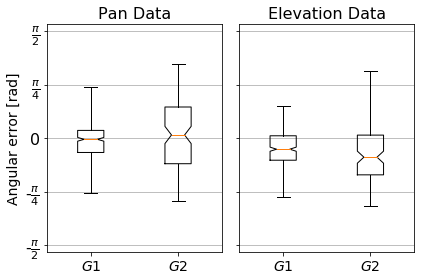
\includegraphics[width=0.7\columnwidth]{figures/pan_tilt_err.png}
  \caption{Boxplots of the angular errors collected during the pointing experiment. }\label{fig:err-results}
\end{figure}

\begin{table}
  \centering
  \caption{A summary of the results collected from the experiment. }\label{tab:results}
  \begin{tabular}{p{1cm}p{2cm}p{4cm}c}
    \toprule
    &           & Mean absolute error [rad]  & Pearson Correlation score \\ \midrule
    \multirow{2}{*}{\textit{G1}} & Pan       & $0.25\pm0.24$ & $0.83\;(p<0.001)$ \\
				 & Elevation & $0.37\pm0.28$ & $0.44\;(p<0.001)$ \\ \midrule
    \multirow{2}{*}{\textit{G2}} & Pan       & $0.38\pm0.21$ & $0.35\;(p<0.001)$ \\
				 & Elevation & $0.51\pm0.32$ & $0.40\;(p=0.001)$ \\
    \bottomrule
  \end{tabular}
\end{table}

The average pan error from group \textit{G1} falls well within the ranges observed in~\cite{macdonald2006spatial,schonstein2008comparison} of $[0.16, 0.38]$ radians and $[0.17, 0.26]$ radians respectively. 
Indeed, the majority of samples fall within even the more conservative latter range. 
However, the participants with vision impairments in group \textit{G2}  demonstrate a wider spread in error data and higher average error than \textit{G1} (0.25 vs. 0.37 radians, Kruskal-Wallis test $p<0.001$). 
The results in~\cite{katz2011spatial,zwiers2001spatial} reported a similar trend, but an investigation with a larger sample size for \textit{G2} should be considered before definitive conclusions can be made.

The elevation estimation performance for both groups deteriorated when compared to their pan estimation results, which was somewhat expected given previous research results on human audition~\cite{barfield1997visual}. 
The mean absolute errors of the participants are \SI{0.37}{\radian} and \SI{0.51}{\radian} for groups \textit{G1} and \textit{G2} respectively.
As with the pan estimation errors, the participants from \textit{G1} seemed more adept at estimating the correct elevation.
%However, the difference is not as significant as for the pan, with \textit{G1} displaying a 36\% improvement over \textit{G2} in their elevation estimation vs. 42.5\% in the pan dimension. 
Comparing these results to methods that convey elevation through an HRTF, we see an improvement of approximately 46\% and 26\% for each group~\cite{schonstein2008comparison}. 
Indeed, the performance is comparable to that of open-back and expensive in-ear headphones.
There is a lesser improvement (11\%) with \textit{G1} when compared to the individualised and adjusted HRTFs in~\cite{stanley2006lateralization} and a 18\% reduction in performance for group \textit{G2}.
However, the participants from~\cite{stanley2006lateralization} all had healthy eyesight, making the latter comparison invalid. 
Interestingly, the elevation errors for group \textit{G2} are centred around the negative angle, indicating a possible underlying bias in the participants or the interface.
A similar trend was observed in~\cite{stanley2006lateralization} and warrants an investigation with a larger participant pool to determine the underlying bias, if any. 

The error data was used to generate scatter plots that show the correlation between the position that the guidance system presented the participants and the position the participants thought the targets were.
These plots are given in \cref{fig:correlation-results} and show a reasonably positive correlation between the guidance targets and the selected targets, which indicates that the participants correctly interpreted the interface's output for the most part. 
The Pearson correlation scores for each dataset, listed in \cref{tab:results}, confirm this.

\begin{figure}[t]
  \centering
  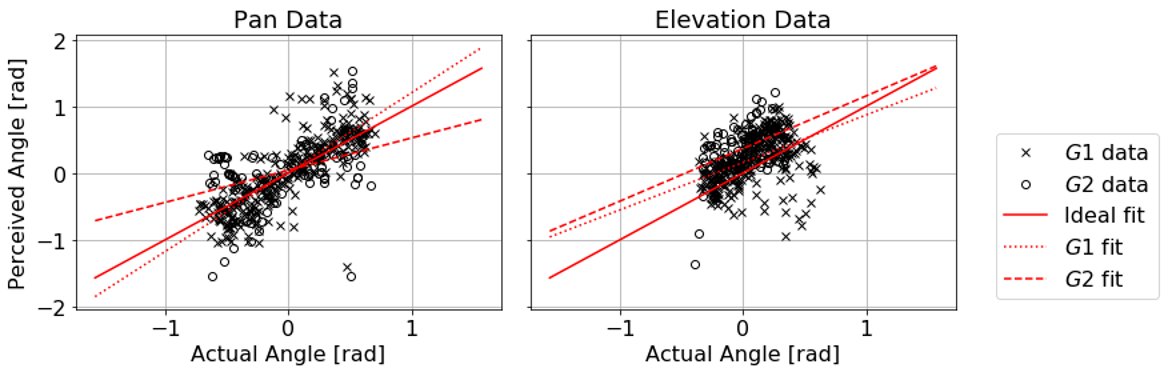
\includegraphics[width=1.0\columnwidth]{figures/correlation.png}
  \caption{Boxplots of the angular errors collected during the pointing experiment. }\label{fig:correlation-results}
\end{figure}

\section{Conclusion}\label{sec:conclusion}

In this work, we proposed an audio interface that conveys a target's pan and elevation angles through a spatialised audio tone that adjusts the tone's pitch to convey the elevation in compensate for the shortcomings of bone-conducting headsets in transmitting the elevation component of a spatialised signal.
Results generated from a simple pointing experiment are encouraging and improves performance over purely spatialised signals transmitted via bone-conduction.
Furthermore, the limitations of these headphones were largely negated by conveying the elevation angle of the target by adjusting the tone's pitch, with pan and elevation errors comparable to that from normal over-ear headphones.

Future work will involve a more in-depth investigation with a larger participant pool to determine the factors that affect performance and enable a more detailed statistical analysis.
For example, will adjusting the elevation function's gradient make it easier to guess the target's elevation and what is the performance difference between participants with limited and healthy eyesight?  
Furthermore, experiments with a large group of people with vision impairments will provide an opportunity to gauge their opinion on the interface and identify possible avenues of improvements to user friendliness.

\bibliographystyle{splncs04}
\bibliography{bib}

\end{document}
